%
%-----------------------------------
\section{Dysprosium}
\label{sec:dysprosium}
%-----------------------------------
%

The dysprosium nMOT \cite{dreon2017optical} reproduced by Davide Dreon and his research group matches the conditions of our experiment and is thoroughly detailed in the Dreon PhD thesis \cite{dreon2017designing}, which helps us improve accuracy as discussed in Section \ref{sec:input-outputs}. Also, our research group is preparing a similar experimental setup in order to study dipolar quantum gases by making use of the large magnetic dipole moment of dysprosium. Moreover, the involved electronic transition presented in Table \ref{tab:electronic-transition-Dy-Dreon} yields a narrowness of $ \eta =  43.8 $ from equation (\ref{eq:narrowness}) and $ R = 169.3 $ from equation (\ref{eq:gravity-radiation-force-ratio}), which are not ideal values. However, the experimental setup is designed to decrease the MOT force in the gravity direction, allowing the atoms to fall under gravity. Therefore, even with a non-ideal narrowness, Dreon nMOT is able to reach the power-broadened regime and then satisfy our model requirements.

\begin{table}[ht!]
    \centering
    \caption{Parameters of the involved electronic transition from the Dreon nMOT.}
    \begin{tabular}{|c|c|c|}
        \hline
        \textbf{Symbol} & \textbf{Quantity} & \textbf{Value} \\ \hline
        $ \Gamma / 2\pi $ & Natural Linewidth & $ 136\ kHz $ \\
        $ \lambda $ & Resonant wavelength & $ 626\ nm $ \\
        $ J_{gnd} $ & Ground state angular momentum & $ 8 $ \\
        $ g_{gnd} $ & Ground state Landé factor & $ 1.24 $ \\
        $ J_{exc} $ & Excited state angular momentum & $ 9 $ \\
        $ g_{exc} $ & Excited state Landé factor & $ 1.29 $ \\
        $ m $ & Mass & $ 164\ u $ \\
        \hline
    \end{tabular}
    \vspace{10px}
    \legend{Source: DREON. \cite{dreon2017designing}.}
    \label{tab:electronic-transition-Dy-Dreon}
\end{table}

The involved transition is more complicated than the one present in Chapter \ref{ch:Monte-Carlo-simulation} since it has 36 possible states in the presence of a magnetic field due to the large angular momenta $ \ket{J = 8} \longrightarrow \ket{J = 9} $. However, in the power-broadened regime, the dysprosium atoms gather in a region with a large and negative magnetic field, which leads to a large and positive Zeeman shift so that an efficient optical pumping populates the absolute ground state $ \ket{J = 8, m_J = -8} $. This spin-polarization was observed experimentally for nMOTs with lanthanide atoms \cite{lu2011strongly,aikawa2012bose} and also in the Dreon experiment. Therefore, due to selection rules (see Appendix \ref{ap:selection-rules}), we can simplify the transitions to a four-level system as illustrated in Figure \ref{fig:Dy-Dreon-electronic-transitions} and then apply our model under the three independent two-level systems assumption.

\begin{figure}[!ht]
    \centering
    \begin{subfigure}[b]{0.48\linewidth}
        \centering
        \subcaption{Electronic transitions}
        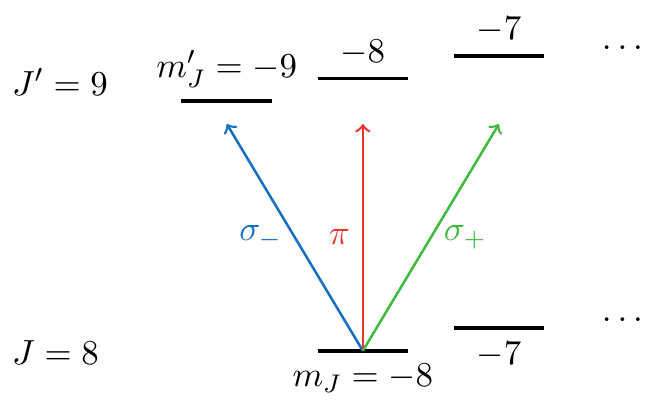
\includegraphics[width=0.8\textwidth]{USPSC-img/Dy-Dreon-transitions.png}
        \label{fig:Dy-Dreon-electronic-transitions}
    \end{subfigure}
    \hfill
    \begin{subfigure}[b]{0.48\linewidth}
        \centering
        \subcaption{Laser beam arrangement}
        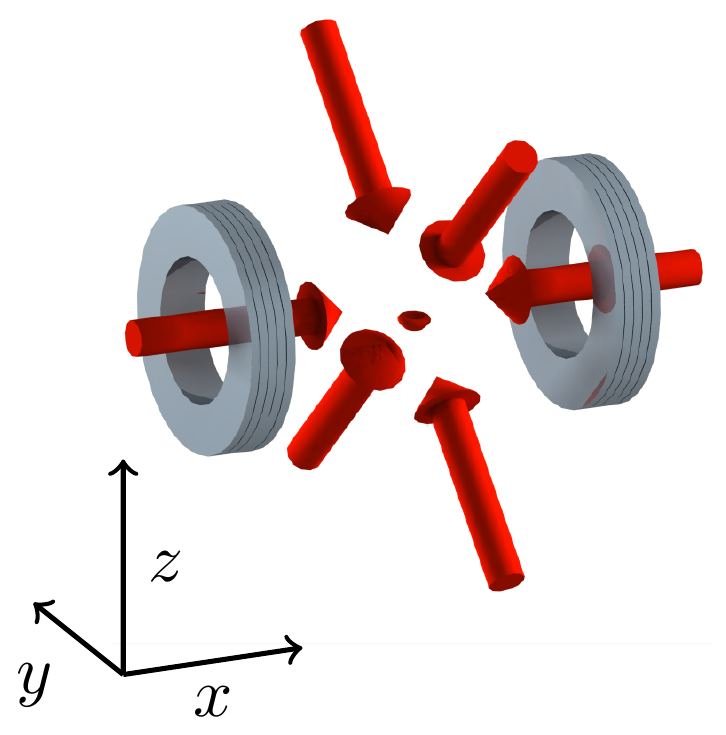
\includegraphics[width=0.6\textwidth]{USPSC-img/Dreon-setup.png}
        \label{fig:Dreon-setup}
    \end{subfigure}
    \vspace{10px}
    \caption{(a) Electronic transitions of spin-polarized dysprosium atoms and (b) laser beam arrangement and Helmholtz coils setup from the Dreon nMOT.}
    \legend{Source: DREON. \textit{et al}. \cite{dreon2017optical}.}
\end{figure}

The arrangement of the lasers is not the usual one introduced in Section \ref{sec:three-dimensional-MOT}, where we have a pair of counter-propagating laser beams in the gravity direction. In the Dreon setup, there are two pairs of counter-propagating laser beams forming an angle of 45 degrees with the gravity direction, as illustrated in Figure \ref{fig:Dreon-setup}. Moreover, the strong and negative magnetic field component is perpendicular to the gravity direction so that the laser beams in this direction have different polarization than the other ones. This setup was designed to decrease the MOT force in the gravity direction and then guarantee that the atoms fall below the magnetic field origin. The parameters of the laser arrangement and the magnetic field profile are presented in Tables \ref{tab:Dreon-laser-beams} and \ref{tab:Dreon-magnetic-field}.

\begin{table}[ht!]
    \centering
    \caption{Wave vector direction $ (x, y, z) $ and polarization $ (\sigma_+, \sigma_-, \pi) $ in the laboratory frame (see Section \ref{sec:magnetic-field-frame}) from Dreon nMOT. All laser beams are set up with the saturation parameter $ s_0 = 0.65 $ and waist $ 2.0\ cm $.}
    \begin{tabular}{|c|c|}
        \hline
        \textbf{Wave vector (arb. unit.)} & \textbf{Polarization} \\ \hline
        $ (1, 0, 0) $ & $ (0, 1, 0) $ \\
        $ (-1, 0, 0) $ & $ (0, 1, 0) $ \\
        $ (0, 1, 1) $ & $ (1, 0, 0) $ \\
        $ (0, -1, 1) $ & $ (1, 0, 0) $ \\
        $ (0, 1, -1) $ & $ (1, 0, 0) $ \\
        $ (0, -1, -1) $ & $ (1, 0, 0) $ \\
        \hline
    \end{tabular}
    \vspace{10px}
    \legend{Source: DREON. \textit{et al}. \cite{dreon2017optical}.}
    \label{tab:Dreon-laser-beams}
\end{table}

\begin{table}[ht!]
    \centering
    \caption{Parameters that defined the magnetic field profile from Dreon nMOT.}
    \begin{tabular}{|c|c|c|}
        \hline
        \textbf{Symbol} & \textbf{Quantity} & \textbf{Value} \\ \hline
        $ B_0 $ & Axial gradient & $ 1.71 G $ \\
        $ B $ & Magnetic Field & $ B_0(-\hat{x} + \hat{y}/2 + \hat{z} / 2) $ \\
        $ B_{bias} $ & Bias & $ (-0.094 \hat{z})\ G / cm $ \\
        \hline
    \end{tabular}
    \vspace{10px}
    \legend{Source: DREON. \textit{et al}. \cite{dreon2017optical}.}
    \label{tab:Dreon-magnetic-field}
\end{table}

%-----------------------------------
\subsection{Atomic cloud profile}
\label{sec:cloud-profile-dysprosium}
%-----------------------------------

The in-situ and estimated atomic cloud profiles are shown in Figures \ref{fig:Dreon-simulated-atomic-cloud-profile} and \ref{fig:Dreon-in-situ-atomic-cloud-profile}. The larger the laser detuning, the lower the centre of mass, and the more spread the atomic cloud. The atomic cloud distributions resemble an ellipsoid whose semi-major axis is perpendicular to the gravity direction. Those are typical effects of power-broadened nMOTs, regardless the slightly large narrowness.

\begin{figure}[!ht]
    \centering
    \begin{subfigure}[b]{0.5\linewidth}
        \centering
        \subcaption{Simulated atomic cloud}
        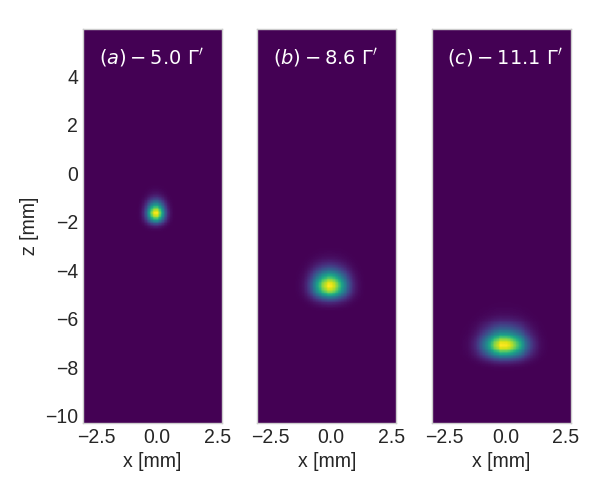
\includegraphics[width=\textwidth]{USPSC-img/dy_dreon_cloud_profile.png}
        \label{fig:Dreon-simulated-atomic-cloud-profile}
    \end{subfigure}
    \hspace{20px}
    \begin{subfigure}[b]{0.4\linewidth}
        \centering
        \subcaption{In-situ atomic cloud}
        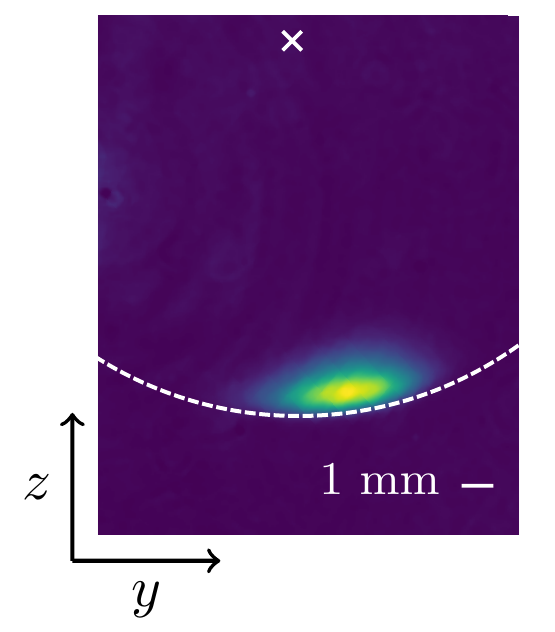
\includegraphics[width=0.7\textwidth]{USPSC-img/in-situ-atomic-cloud-Dreon.png}
        \vspace{30px}
        \label{fig:Dreon-in-situ-atomic-cloud-profile}
    \end{subfigure}
    \caption{(a) Estimated atomic cloud profile for different laser detunings based on equation (\ref{eq:joint-position-distribution}). (b) In-situ atomic cloud profiles from the Dreon nMOT.}
    \legend{Source (a): By the author; (b): DREON. \textit{et al}. \cite{dreon2017optical}.}
\end{figure}

From equation (\ref{eq:centre-of-mass-power-broadened-regime}), we expect that the centre of mass\footnote{We are considering only the z component as the centre of mass since all other components is about zero in all cases.} of the atomic cloud is proportional to the laser detuning for large detunings. In fact, the estimated centre of mass given by equation (\ref{eq:simulated-centre-of-mass}) and the experimental measures confirm this linear relation for laser detunings roughly larger than $ 2\pi \times 700\ kHz \simeq 4\Gamma' $, as illustrated in Figure \ref{fig:Dreon-centre-of-mass}. However, the theoretical centre of mass is not as accurate as the estimated one since there is a difference of about $1mm$ between the experimental and theoretical centre of mass, whereas the estimated values match almost perfectly the experimental measures.

\begin{figure}[!ht]
    \centering
    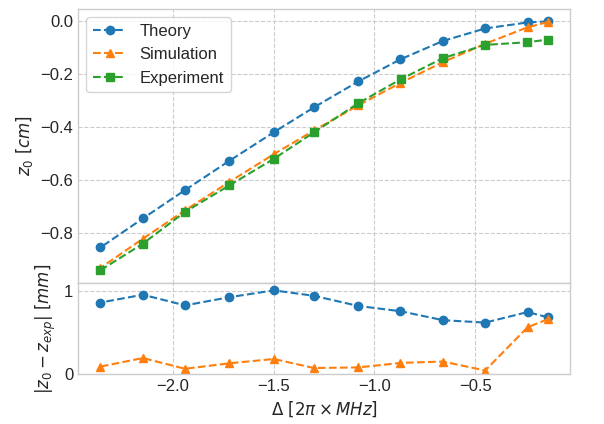
\includegraphics[width=0.6\textwidth]{USPSC-img/dy_centre_of_mass.png}
    \vspace{5px}
    \caption{The gravity direction component of the centre of mass as a function of the laser detuning. The blue spheres, orange triangles, and green squares are, respectively, the theoretical centres of mass from equation (\ref{eq:centre-of-mass-power-broadened-regime}), estimated points, and experimental measures from \cite{dreon2017designing}.}
    \legend{Source: By the author.}
    \label{fig:Dreon-centre-of-mass}
\end{figure}

We do not expect an accurate estimative of the cloud size since this quantity is affected by interactions between atoms, which are not taken into account in our model. Indeed, the experimental cloud sized is larger than the estimated ones given by equation (\ref{eq:simulated-cloud-sizes}), as illustrated in Figure \ref{fig:Dreon-cloud-size}. This is expected due to the re-absorption of scattered photons. Nevertheless, we are able to compare the experimental and estimated cloud sizes more clearly by verifying the ratio between two cloud size components, as illustrated in Figure \ref{fig:Dreon-cloud-size-ratio}. It was observed in previous works \cite{PhysRevA.90.063404} that the cloud size is proportional to the cube root of the number of trapped atoms $ \sqrt[3]{N} $ as discussed in Section \ref{sec:MOT-cloud-size}. Therefore, we remove the effect of scaling constants by analysing the ratio between components. The experimental and estimated cloud sizes match roughly in the laser detuning range of $ -10\Gamma' $ to $ -4\Gamma' $ ($ -2\pi \times 1750 kHz $ to $ -2\pi \times 700 kHz $). We expect that the estimated cloud sizes do not match the experimental ones for lower detunings (in module) because we are out of the power-broadened regime. Although there are no experimental measures available in this range, we can observe that there are variations inconsistent with the range in which there is agreement between experimental and estimated values. For laser detunings larger than $ 10\Gamma' $ in module, we do not have a good matching mostly due to the $ \sigma_y $ values. To explain such divergence, we must consider that an ellipsoid bounds the region in which the atoms can be trapped. The curvature effect is particularly predominant in the x and y directions and can invalidate the scaling factor $ \sqrt[3]{N} $.

\begin{figure}[!ht]
    \centering
    \begin{subfigure}[b]{0.5\linewidth}
        \centering
        \subcaption{Cloud sizes $ \sigma_y $ and $ \sigma_z $}
        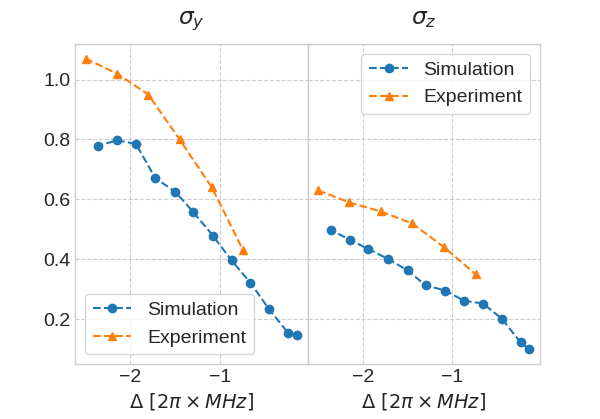
\includegraphics[width=\textwidth]{USPSC-img/dy_cloud_size.png}
        \label{fig:Dreon-cloud-size}
    \end{subfigure}
    \hfill
    \begin{subfigure}[b]{0.45\linewidth}
        \centering
        \subcaption{Cloud size ratio $ \sigma_y / \sigma_z $}
        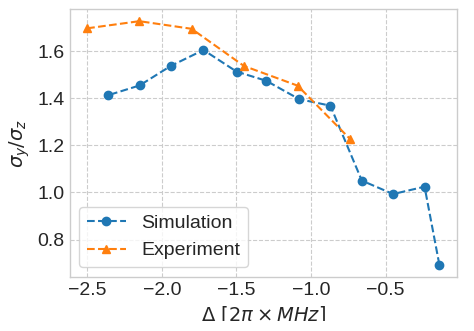
\includegraphics[width=\textwidth]{USPSC-img/dy_cloud_size_ratio.png}
        \label{fig:Dreon-cloud-size-ratio}
    \end{subfigure}
    \caption{(a) Cloud sizes $ \sigma_y $ and $ \sigma_z $ and (b) cloud ratio $ \sigma_y / \sigma_z $ as a function of the laser detuning. The blue spheres and orange triangles are the estimated and experimental cloud sizes respectively.}
    \legend{Source: By the author.}
\end{figure}

%-----------------------------------
\subsection{Temperature}
\label{temperature}
%-----------------------------------

The experimental and estimated temperatures are shown in Figure \ref{fig:Dreon-temperature}. Firstly, both estimated and experimental temperatures are higher than the theoretical temperature $ T_D = 4.19\ \mu K $ given by equation (\ref{eq:Doppler-temperature-high-saturation}). For laser detunings roughly larger than $ 6 \Gamma' \simeq 7.5 \Gamma $ in module, the experimental measures match the estimated values. In this range, the temperature is approximately constant, which agrees with the theoretical temperature given by equation (\ref{eq:Doppler-temperature-high-saturation}). However, the absolute theoretical value does not match the experimental measures. For detunings roughly lower than $ 6 \Gamma' $, the experimental temperatures increases with the laser detuning whereas the estimated values decreases. In this range, the nMOT is not in the power-broadened regime.

\begin{figure}[!ht]
    \centering
    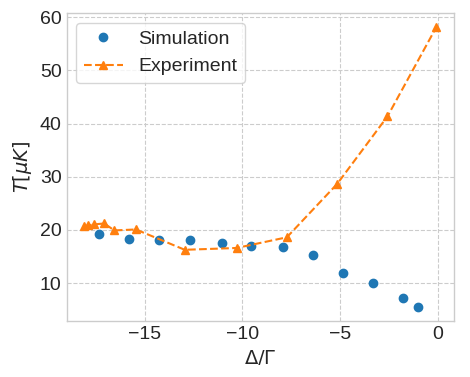
\includegraphics[width=0.45\textwidth]{USPSC-img/dy_temperature.png}
    \vspace{5px}
    \caption{Temperature of the Dreon nMOT as a function of the laser detuning. The blue spheres and the orange triangles are the estimated and experimental temperatures respectively. We can roughly split the temperatures into two regions at the laser detuning $ -6 \Gamma' \simeq 7.5 \Gamma $. For detunings lower than $ 6 \Gamma'  $ in module, the nMOT is not in the power-broadened regime and then present a divergence between experimental and estimated values.}
    \legend{Source: By the author.}
    \label{fig:Dreon-temperature}
\end{figure}
